\documentclass[1p]{elsarticle_modified}
%\bibliographystyle{elsarticle-num}

%\usepackage[colorlinks]{hyperref}
%\usepackage{abbrmath_seonhwa} %\Abb, \Ascr, \Acal ,\Abf, \Afrak
\usepackage{amsfonts}
\usepackage{amssymb}
\usepackage{amsmath}
\usepackage{amsthm}
\usepackage{scalefnt}
\usepackage{amsbsy}
\usepackage{kotex}
\usepackage{caption}
\usepackage{subfig}
\usepackage{color}
\usepackage{graphicx}
\usepackage{xcolor} %% white, black, red, green, blue, cyan, magenta, yellow
\usepackage{float}
\usepackage{setspace}
\usepackage{hyperref}

\usepackage{tikz}
\usetikzlibrary{arrows}

\usepackage{multirow}
\usepackage{array} % fixed length table
\usepackage{hhline}

%%%%%%%%%%%%%%%%%%%%%
\makeatletter
\renewcommand*\env@matrix[1][\arraystretch]{%
	\edef\arraystretch{#1}%
	\hskip -\arraycolsep
	\let\@ifnextchar\new@ifnextchar
	\array{*\c@MaxMatrixCols c}}
\makeatother %https://tex.stackexchange.com/questions/14071/how-can-i-increase-the-line-spacing-in-a-matrix
%%%%%%%%%%%%%%%

\usepackage[normalem]{ulem}

\newcommand{\msout}[1]{\ifmmode\text{\sout{\ensuremath{#1}}}\else\sout{#1}\fi}
%SOURCE: \msout is \stkout macro in https://tex.stackexchange.com/questions/20609/strikeout-in-math-mode

\newcommand{\cancel}[1]{
	\ifmmode
	{\color{red}\msout{#1}}
	\else
	{\color{red}\sout{#1}}
	\fi
}

\newcommand{\add}[1]{
	{\color{blue}\uwave{#1}}
}

\newcommand{\replace}[2]{
	\ifmmode
	{\color{red}\msout{#1}}{\color{blue}\uwave{#2}}
	\else
	{\color{red}\sout{#1}}{\color{blue}\uwave{#2}}
	\fi
}

\newcommand{\Sol}{\mathcal{S}} %segment
\newcommand{\D}{D} %diagram
\newcommand{\A}{\mathcal{A}} %arc


%%%%%%%%%%%%%%%%%%%%%%%%%%%%%5 test

\def\sl{\operatorname{\textup{SL}}(2,\Cbb)}
\def\psl{\operatorname{\textup{PSL}}(2,\Cbb)}
\def\quan{\mkern 1mu \triangleright \mkern 1mu}

\theoremstyle{definition}
\newtheorem{thm}{Theorem}[section]
\newtheorem{prop}[thm]{Proposition}
\newtheorem{lem}[thm]{Lemma}
\newtheorem{ques}[thm]{Question}
\newtheorem{cor}[thm]{Corollary}
\newtheorem{defn}[thm]{Definition}
\newtheorem{exam}[thm]{Example}
\newtheorem{rmk}[thm]{Remark}
\newtheorem{alg}[thm]{Algorithm}

\newcommand{\I}{\sqrt{-1}}
\begin{document}

%\begin{frontmatter}
%
%\title{Boundary parabolic representations of knots up to 8 crossings}
%
%%% Group authors per affiliation:
%\author{Yunhi Cho} 
%\address{Department of Mathematics, University of Seoul, Seoul, Korea}
%\ead{yhcho@uos.ac.kr}
%
%
%\author{Seonhwa Kim} %\fnref{s_kim}}
%\address{Center for Geometry and Physics, Institute for Basic Science, Pohang, 37673, Korea}
%\ead{ryeona17@ibs.re.kr}
%
%\author{Hyuk Kim}
%\address{Department of Mathematical Sciences, Seoul National University, Seoul 08826, Korea}
%\ead{hyukkim@snu.ac.kr}
%
%\author{Seokbeom Yoon}
%\address{Department of Mathematical Sciences, Seoul National University, Seoul, 08826,  Korea}
%\ead{sbyoon15@snu.ac.kr}
%
%\begin{abstract}
%We find all boundary parabolic representation of knots up to 8 crossings.
%
%\end{abstract}
%\begin{keyword}
%    \MSC[2010] 57M25 
%\end{keyword}
%
%\end{frontmatter}

%\linenumbers
%\tableofcontents
%
\newcommand\colored[1]{\textcolor{white}{\rule[-0.35ex]{0.8em}{1.4ex}}\kern-0.8em\color{red} #1}%
%\newcommand\colored[1]{\textcolor{white}{ #1}\kern-2.17ex	\textcolor{white}{ #1}\kern-1.81ex	\textcolor{white}{ #1}\kern-2.15ex\color{red}#1	}

{\Large $\underline{12n_{0279}~(K12n_{0279})}$}

\setlength{\tabcolsep}{10pt}
\renewcommand{\arraystretch}{1.6}
\vspace{1cm}\begin{tabular}{m{100pt}>{\centering\arraybackslash}m{274pt}}
\multirow{5}{120pt}{
	\centering
	\includegraphics[width=112pt]{../../../GIT/diagram.site/Diagrams/png/2368_12n_0279.png}\\
\ \ \ A knot diagram\footnotemark}&
\allowdisplaybreaks
\textbf{Linearized knot diagam} \\
\cline{2-2}
 &
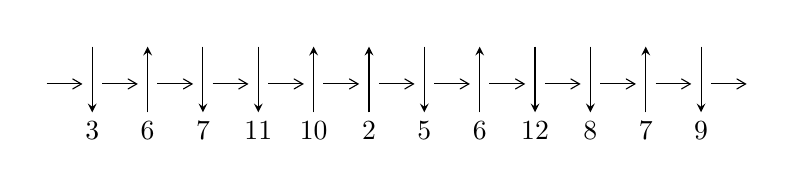
\begin{tikzpicture}[x=20pt, y=17pt]
	% nodes
	\node (C0) at (0, 0) {};
	\node (C1) at (1, 0) {};
	\node (C1U) at (1, +1) {};
	\node (C1D) at (1, -1) {3};

	\node (C2) at (2, 0) {};
	\node (C2U) at (2, +1) {};
	\node (C2D) at (2, -1) {6};

	\node (C3) at (3, 0) {};
	\node (C3U) at (3, +1) {};
	\node (C3D) at (3, -1) {7};

	\node (C4) at (4, 0) {};
	\node (C4U) at (4, +1) {};
	\node (C4D) at (4, -1) {11};

	\node (C5) at (5, 0) {};
	\node (C5U) at (5, +1) {};
	\node (C5D) at (5, -1) {10};

	\node (C6) at (6, 0) {};
	\node (C6U) at (6, +1) {};
	\node (C6D) at (6, -1) {2};

	\node (C7) at (7, 0) {};
	\node (C7U) at (7, +1) {};
	\node (C7D) at (7, -1) {5};

	\node (C8) at (8, 0) {};
	\node (C8U) at (8, +1) {};
	\node (C8D) at (8, -1) {6};

	\node (C9) at (9, 0) {};
	\node (C9U) at (9, +1) {};
	\node (C9D) at (9, -1) {12};

	\node (C10) at (10, 0) {};
	\node (C10U) at (10, +1) {};
	\node (C10D) at (10, -1) {8};

	\node (C11) at (11, 0) {};
	\node (C11U) at (11, +1) {};
	\node (C11D) at (11, -1) {7};

	\node (C12) at (12, 0) {};
	\node (C12U) at (12, +1) {};
	\node (C12D) at (12, -1) {9};
	\node (C13) at (13, 0) {};

	% arrows
	\draw[->,>={angle 60}]
	(C0) edge (C1) (C1) edge (C2) (C2) edge (C3) (C3) edge (C4) (C4) edge (C5) (C5) edge (C6) (C6) edge (C7) (C7) edge (C8) (C8) edge (C9) (C9) edge (C10) (C10) edge (C11) (C11) edge (C12) (C12) edge (C13) ;	\draw[->,>=stealth]
	(C1U) edge (C1D) (C2D) edge (C2U) (C3U) edge (C3D) (C4U) edge (C4D) (C5D) edge (C5U) (C6D) edge (C6U) (C7U) edge (C7D) (C8D) edge (C8U) (C9U) edge (C9D) (C10U) edge (C10D) (C11D) edge (C11U) (C12U) edge (C12D) ;
	\end{tikzpicture} \\
\hhline{~~} \\& 
\textbf{Solving Sequence} \\ \cline{2-2} 
 &
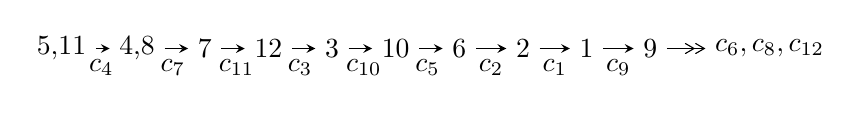
\begin{tikzpicture}[x=23pt, y=7pt]
	% node
	\node (A0) at (-1/8, 0) {5,11};
	\node (A1) at (17/16, 0) {4,8};
	\node (A2) at (17/8, 0) {7};
	\node (A3) at (25/8, 0) {12};
	\node (A4) at (33/8, 0) {3};
	\node (A5) at (41/8, 0) {10};
	\node (A6) at (49/8, 0) {6};
	\node (A7) at (57/8, 0) {2};
	\node (A8) at (65/8, 0) {1};
	\node (A9) at (73/8, 0) {9};
	\node (C1) at (1/2, -1) {$c_{4}$};
	\node (C2) at (13/8, -1) {$c_{7}$};
	\node (C3) at (21/8, -1) {$c_{11}$};
	\node (C4) at (29/8, -1) {$c_{3}$};
	\node (C5) at (37/8, -1) {$c_{10}$};
	\node (C6) at (45/8, -1) {$c_{5}$};
	\node (C7) at (53/8, -1) {$c_{2}$};
	\node (C8) at (61/8, -1) {$c_{1}$};
	\node (C9) at (69/8, -1) {$c_{9}$};
	\node (A10) at (11, 0) {$c_{6},c_{8},c_{12}$};

	% edge
	\draw[->,>=stealth]	
	(A0) edge (A1) (A1) edge (A2) (A2) edge (A3) (A3) edge (A4) (A4) edge (A5) (A5) edge (A6) (A6) edge (A7) (A7) edge (A8) (A8) edge (A9) ;
	\draw[->>,>={angle 60}]	
	(A9) edge (A10);
\end{tikzpicture} \\ 

\end{tabular} \\

\footnotetext{
The image of knot diagram is generated by the software ``\textbf{Draw programme}" developed by Andrew Bartholomew(\url{http://www.layer8.co.uk/maths/draw/index.htm\#Running-draw}), where we modified some parts for our purpose(\url{https://github.com/CATsTAILs/LinksPainter}).
}\phantom \\ \newline 
\centering \textbf{Ideals for irreducible components\footnotemark of $X_{\text{par}}$} 
 
\begin{align*}
I^u_{1}&=\langle 
27831408 u^{16}+38249416 u^{15}+\cdots+40002991 b+40510496,\\
\phantom{I^u_{1}}&\phantom{= \langle  }-24958754 u^{16}-42710149 u^{15}+\cdots+40002991 a-62762092,\;u^{17}+u^{16}+\cdots+u-1\rangle \\
I^u_{2}&=\langle 
b+u+1,\;u^2+a-1,\;u^3+u^2+1\rangle \\
I^u_{3}&=\langle 
- u^3+b- u,\;a+u+1,\;u^4- u^3+2 u^2-2 u+1\rangle \\
I^u_{4}&=\langle 
- u^3+b-2 u-1,\;a,\;u^4- u^3+3 u^2- u+1\rangle \\
I^u_{5}&=\langle 
- a u+3 b+a+3 u,\;a^2+a u- a-3,\;u^2+u+1\rangle \\
I^u_{6}&=\langle 
-2.19461\times10^{15} u^{13}-2.90056\times10^{15} u^{12}+\cdots+6.79307\times10^{17} b-2.81232\times10^{17},\\
\phantom{I^u_{6}}&\phantom{= \langle  }-3.53923\times10^{17} u^{13}-5.35522\times10^{17} u^{12}+\cdots+7.20066\times10^{19} a-1.96602\times10^{20},\\
\phantom{I^u_{6}}&\phantom{= \langle  }u^{14}+u^{13}+\cdots-98 u+53\rangle \\
I^u_{7}&=\langle 
b-1,\;a,\;u^2+u+1\rangle \\
I^u_{8}&=\langle 
b- u,\;a,\;u^2+u+1\rangle \\
\\
\end{align*}
\raggedright * 8 irreducible components of $\dim_{\mathbb{C}}=0$, with total 50 representations.\\
\footnotetext{All coefficients of polynomials are rational numbers. But the coefficients are sometimes approximated in decimal forms when there is not enough margin.}
\newpage
\renewcommand{\arraystretch}{1}
\centering \section*{I. $I^u_{1}= \langle 2.78\times10^{7} u^{16}+3.82\times10^{7} u^{15}+\cdots+4.00\times10^{7} b+4.05\times10^{7},\;-2.50\times10^{7} u^{16}-4.27\times10^{7} u^{15}+\cdots+4.00\times10^{7} a-6.28\times10^{7},\;u^{17}+u^{16}+\cdots+u-1 \rangle$}
\flushleft \textbf{(i) Arc colorings}\\
\begin{tabular}{m{7pt} m{180pt} m{7pt} m{180pt} }
\flushright $a_{5}=$&$\begin{pmatrix}1\\0\end{pmatrix}$ \\
\flushright $a_{11}=$&$\begin{pmatrix}0\\u\end{pmatrix}$ \\
\flushright $a_{4}=$&$\begin{pmatrix}1\\- u^2\end{pmatrix}$ \\
\flushright $a_{8}=$&$\begin{pmatrix}0.623922 u^{16}+1.06767 u^{15}+\cdots-4.19761 u+1.56893\\-0.695733 u^{16}-0.956164 u^{15}+\cdots+4.01744 u-1.01269\end{pmatrix}$ \\
\flushright $a_{7}=$&$\begin{pmatrix}-0.0718110 u^{16}+0.111510 u^{15}+\cdots-0.180171 u+0.556248\\-0.695733 u^{16}-0.956164 u^{15}+\cdots+4.01744 u-1.01269\end{pmatrix}$ \\
\flushright $a_{12}=$&$\begin{pmatrix}0.463872 u^{16}+0.672655 u^{15}+\cdots+0.262187 u-0.138788\\-0.152299 u^{16}-0.109999 u^{15}+\cdots+0.667583 u-0.892029\end{pmatrix}$ \\
\flushright $a_{3}=$&$\begin{pmatrix}0.683246 u^{16}+1.06132 u^{15}+\cdots-4.69765 u+1.76057\\-0.917110 u^{16}-0.866468 u^{15}+\cdots+2.11890 u-0.443964\end{pmatrix}$ \\
\flushright $a_{10}=$&$\begin{pmatrix}0.664842 u^{16}+0.607334 u^{15}+\cdots+0.648473 u+2.52008\\-0.0486712 u^{16}+0.175319 u^{15}+\cdots+0.946131 u-1.76684\end{pmatrix}$ \\
\flushright $a_{6}=$&$\begin{pmatrix}-1.82038 u^{16}-2.59604 u^{15}+\cdots+4.42105 u+1.28803\\0.390419 u^{16}+0.580544 u^{15}+\cdots+0.744719 u+0.433797\end{pmatrix}$ \\
\flushright $a_{2}=$&$\begin{pmatrix}0.842480 u^{16}+0.955949 u^{15}+\cdots+0.0116457 u+2.65839\\-0.369554 u^{16}+0.163720 u^{15}+\cdots-0.697278 u-1.38144\end{pmatrix}$ \\
\flushright $a_{1}=$&$\begin{pmatrix}-0.295603 u^{16}-0.654268 u^{15}+\cdots+1.33796 u+0.594847\\0.323305 u^{16}+0.418596 u^{15}+\cdots-2.19115 u+0.801058\end{pmatrix}$ \\
\flushright $a_{9}=$&$\begin{pmatrix}0.456059 u^{16}+0.624327 u^{15}+\cdots+1.25113 u+2.05621\\-0.0909712 u^{16}+0.0800344 u^{15}+\cdots+1.68586 u-1.61454\end{pmatrix}$\\&\end{tabular}
\flushleft \textbf{(ii) Obstruction class $= -1$}\\~\\
\flushleft \textbf{(iii) Cusp Shapes $= -\frac{217036647}{40002991} u^{16}-\frac{332499894}{40002991} u^{15}+\cdots+\frac{1336970457}{40002991} u+\frac{36116891}{40002991}$}\\~\\
\newpage\renewcommand{\arraystretch}{1}
\flushleft \textbf{(iv) u-Polynomials at the component}\newline \\
\begin{tabular}{m{50pt}|m{274pt}}
Crossings & \hspace{64pt}u-Polynomials at each crossing \\
\hline $$\begin{aligned}c_{1}\end{aligned}$$&$\begin{aligned}
&u^{17}+8 u^{16}+\cdots-2 u-1
\end{aligned}$\\
\hline $$\begin{aligned}c_{2},c_{5},c_{6}\end{aligned}$$&$\begin{aligned}
&u^{17}+4 u^{15}+\cdots+2 u+1
\end{aligned}$\\
\hline $$\begin{aligned}c_{3}\end{aligned}$$&$\begin{aligned}
&u^{17}+3 u^{16}+\cdots+96 u+29
\end{aligned}$\\
\hline $$\begin{aligned}c_{4},c_{9},c_{12}\end{aligned}$$&$\begin{aligned}
&u^{17}- u^{16}+\cdots+u+1
\end{aligned}$\\
\hline $$\begin{aligned}c_{7}\end{aligned}$$&$\begin{aligned}
&u^{17}-2 u^{16}+\cdots+4 u-1
\end{aligned}$\\
\hline $$\begin{aligned}c_{8}\end{aligned}$$&$\begin{aligned}
&u^{17}+4 u^{16}+\cdots+358 u-23
\end{aligned}$\\
\hline $$\begin{aligned}c_{10}\end{aligned}$$&$\begin{aligned}
&u^{17}-2 u^{16}+\cdots-8 u+4
\end{aligned}$\\
\hline $$\begin{aligned}c_{11}\end{aligned}$$&$\begin{aligned}
&u^{17}- u^{16}+\cdots+192 u+79
\end{aligned}$\\
\hline
\end{tabular}\\~\\
\newpage\renewcommand{\arraystretch}{1}
\flushleft \textbf{(v) Riley Polynomials at the component}\newline \\
\begin{tabular}{m{50pt}|m{274pt}}
Crossings & \hspace{64pt}Riley Polynomials at each crossing \\
\hline $$\begin{aligned}c_{1}\end{aligned}$$&$\begin{aligned}
&y^{17}+36 y^{16}+\cdots+70 y-1
\end{aligned}$\\
\hline $$\begin{aligned}c_{2},c_{5},c_{6}\end{aligned}$$&$\begin{aligned}
&y^{17}+8 y^{16}+\cdots-2 y-1
\end{aligned}$\\
\hline $$\begin{aligned}c_{3}\end{aligned}$$&$\begin{aligned}
&y^{17}+31 y^{16}+\cdots-13636 y-841
\end{aligned}$\\
\hline $$\begin{aligned}c_{4},c_{9},c_{12}\end{aligned}$$&$\begin{aligned}
&y^{17}+21 y^{16}+\cdots-21 y-1
\end{aligned}$\\
\hline $$\begin{aligned}c_{7}\end{aligned}$$&$\begin{aligned}
&y^{17}+18 y^{15}+\cdots-10 y-1
\end{aligned}$\\
\hline $$\begin{aligned}c_{8}\end{aligned}$$&$\begin{aligned}
&y^{17}-36 y^{16}+\cdots+196750 y-529
\end{aligned}$\\
\hline $$\begin{aligned}c_{10}\end{aligned}$$&$\begin{aligned}
&y^{17}+8 y^{16}+\cdots+96 y-16
\end{aligned}$\\
\hline $$\begin{aligned}c_{11}\end{aligned}$$&$\begin{aligned}
&y^{17}-33 y^{16}+\cdots-62044 y-6241
\end{aligned}$\\
\hline
\end{tabular}\\~\\
\newpage\flushleft \textbf{(vi) Complex Volumes and Cusp Shapes}
$$\begin{array}{c|c|c}  
\text{Solutions to }I^u_{1}& \I (\text{vol} + \sqrt{-1}CS) & \text{Cusp shape}\\
 \hline 
\begin{aligned}
u &= -0.057958 + 1.037160 I \\
a &= -1.281730 - 0.156187 I \\
b &= -0.146308 - 0.285619 I\end{aligned}
 & \phantom{-}0.90500 - 3.77030 I & \phantom{-}1.82474 + 3.48475 I \\ \hline\begin{aligned}
u &= -0.057958 - 1.037160 I \\
a &= -1.281730 + 0.156187 I \\
b &= -0.146308 + 0.285619 I\end{aligned}
 & \phantom{-}0.90500 + 3.77030 I & \phantom{-}1.82474 - 3.48475 I \\ \hline\begin{aligned}
u &= \phantom{-}0.245125 + 1.028970 I \\
a &= -1.09741 + 0.90076 I \\
b &= \phantom{-}0.457121 + 1.056880 I\end{aligned}
 & \phantom{-}4.13880 - 5.40035 I & \phantom{-}4.91651 + 8.34008 I \\ \hline\begin{aligned}
u &= \phantom{-}0.245125 - 1.028970 I \\
a &= -1.09741 - 0.90076 I \\
b &= \phantom{-}0.457121 - 1.056880 I\end{aligned}
 & \phantom{-}4.13880 + 5.40035 I & \phantom{-}4.91651 - 8.34008 I \\ \hline\begin{aligned}
u &= -0.397934 + 0.813970 I \\
a &= -0.976997 - 0.362526 I \\
b &= \phantom{-}1.21505 - 1.10098 I\end{aligned}
 & -0.17756 + 4.89986 I & -2.88050 - 11.83276 I \\ \hline\begin{aligned}
u &= -0.397934 - 0.813970 I \\
a &= -0.976997 + 0.362526 I \\
b &= \phantom{-}1.21505 + 1.10098 I\end{aligned}
 & -0.17756 - 4.89986 I & -2.88050 + 11.83276 I \\ \hline\begin{aligned}
u &= \phantom{-}0.355960 + 0.790874 I \\
a &= -0.144449 + 0.440961 I \\
b &= \phantom{-}0.821906 + 0.423349 I\end{aligned}
 & -0.33729 - 2.00763 I & -4.27790 + 4.10487 I \\ \hline\begin{aligned}
u &= \phantom{-}0.355960 - 0.790874 I \\
a &= -0.144449 - 0.440961 I \\
b &= \phantom{-}0.821906 - 0.423349 I\end{aligned}
 & -0.33729 + 2.00763 I & -4.27790 - 4.10487 I \\ \hline\begin{aligned}
u &= \phantom{-}1.21780\phantom{ +0.000000I} \\
a &= \phantom{-}1.23271\phantom{ +0.000000I} \\
b &= -0.577819\phantom{ +0.000000I}\end{aligned}
 & -2.39027\phantom{ +0.000000I} & -14.2090\phantom{ +0.000000I} \\ \hline\begin{aligned}
u &= \phantom{-}0.299458 + 0.466008 I \\
a &= \phantom{-}2.32811 + 0.28399 I \\
b &= -1.079530 - 0.618458 I\end{aligned}
 & -3.08489 - 6.04547 I & -8.76917 + 6.36123 I\\
 \hline 
 \end{array}$$\newpage$$\begin{array}{c|c|c}  
\text{Solutions to }I^u_{1}& \I (\text{vol} + \sqrt{-1}CS) & \text{Cusp shape}\\
 \hline 
\begin{aligned}
u &= \phantom{-}0.299458 - 0.466008 I \\
a &= \phantom{-}2.32811 - 0.28399 I \\
b &= -1.079530 + 0.618458 I\end{aligned}
 & -3.08489 + 6.04547 I & -8.76917 - 6.36123 I \\ \hline\begin{aligned}
u &= -0.108066 + 0.363788 I \\
a &= \phantom{-}0.949976 - 0.957388 I \\
b &= \phantom{-}0.119264 + 0.837933 I\end{aligned}
 & \phantom{-}0.52238 - 1.49726 I & \phantom{-}2.87825 + 5.01467 I \\ \hline\begin{aligned}
u &= -0.108066 - 0.363788 I \\
a &= \phantom{-}0.949976 + 0.957388 I \\
b &= \phantom{-}0.119264 - 0.837933 I\end{aligned}
 & \phantom{-}0.52238 + 1.49726 I & \phantom{-}2.87825 - 5.01467 I \\ \hline\begin{aligned}
u &= -0.71553 + 2.03646 I \\
a &= \phantom{-}0.617685 + 0.005897 I \\
b &= -1.02465 - 1.09864 I\end{aligned}
 & \phantom{-}17.8274 + 5.4627 I & -0.12519 - 2.24848 I \\ \hline\begin{aligned}
u &= -0.71553 - 2.03646 I \\
a &= \phantom{-}0.617685 - 0.005897 I \\
b &= -1.02465 + 1.09864 I\end{aligned}
 & \phantom{-}17.8274 - 5.4627 I & -0.12519 + 2.24848 I \\ \hline\begin{aligned}
u &= -0.72995 + 2.19477 I \\
a &= \phantom{-}0.988459 + 0.323341 I \\
b &= -1.07394 + 1.02493 I\end{aligned}
 & \phantom{-}17.5899 + 13.2299 I & -0.46218 - 5.67701 I \\ \hline\begin{aligned}
u &= -0.72995 - 2.19477 I \\
a &= \phantom{-}0.988459 - 0.323341 I \\
b &= -1.07394 - 1.02493 I\end{aligned}
 & \phantom{-}17.5899 - 13.2299 I & -0.46218 + 5.67701 I\\
 \hline 
 \end{array}$$\newpage\newpage\renewcommand{\arraystretch}{1}
\centering \section*{II. $I^u_{2}= \langle b+u+1,\;u^2+a-1,\;u^3+u^2+1 \rangle$}
\flushleft \textbf{(i) Arc colorings}\\
\begin{tabular}{m{7pt} m{180pt} m{7pt} m{180pt} }
\flushright $a_{5}=$&$\begin{pmatrix}1\\0\end{pmatrix}$ \\
\flushright $a_{11}=$&$\begin{pmatrix}0\\u\end{pmatrix}$ \\
\flushright $a_{4}=$&$\begin{pmatrix}1\\- u^2\end{pmatrix}$ \\
\flushright $a_{8}=$&$\begin{pmatrix}- u^2+1\\- u-1\end{pmatrix}$ \\
\flushright $a_{7}=$&$\begin{pmatrix}- u^2- u\\- u-1\end{pmatrix}$ \\
\flushright $a_{12}=$&$\begin{pmatrix}- u^2- u\\-1\end{pmatrix}$ \\
\flushright $a_{3}=$&$\begin{pmatrix}- u^2- u+1\\- u^2- u-1\end{pmatrix}$ \\
\flushright $a_{10}=$&$\begin{pmatrix}2 u+1\\- u^2- u\end{pmatrix}$ \\
\flushright $a_{6}=$&$\begin{pmatrix}u^2+u-1\\u+1\end{pmatrix}$ \\
\flushright $a_{2}=$&$\begin{pmatrix}u+2\\-2 u^2-2 u\end{pmatrix}$ \\
\flushright $a_{1}=$&$\begin{pmatrix}u^2+u\\- u^2\end{pmatrix}$ \\
\flushright $a_{9}=$&$\begin{pmatrix}2 u+2\\- u^2-2 u\end{pmatrix}$\\&\end{tabular}
\flushleft \textbf{(ii) Obstruction class $= 1$}\\~\\
\flushleft \textbf{(iii) Cusp Shapes $= 8 u^2+7 u+3$}\\~\\
\newpage\renewcommand{\arraystretch}{1}
\flushleft \textbf{(iv) u-Polynomials at the component}\newline \\
\begin{tabular}{m{50pt}|m{274pt}}
Crossings & \hspace{64pt}u-Polynomials at each crossing \\
\hline $$\begin{aligned}c_{1},c_{7}\end{aligned}$$&$\begin{aligned}
&u^3-2 u^2+u+1
\end{aligned}$\\
\hline $$\begin{aligned}c_{2},c_{5}\end{aligned}$$&$\begin{aligned}
&u^3+u+1
\end{aligned}$\\
\hline $$\begin{aligned}c_{3},c_{11}\end{aligned}$$&$\begin{aligned}
&(u+1)^3
\end{aligned}$\\
\hline $$\begin{aligned}c_{4},c_{12}\end{aligned}$$&$\begin{aligned}
&u^3+u^2+1
\end{aligned}$\\
\hline $$\begin{aligned}c_{6},c_{8}\end{aligned}$$&$\begin{aligned}
&u^3+u-1
\end{aligned}$\\
\hline $$\begin{aligned}c_{9}\end{aligned}$$&$\begin{aligned}
&u^3- u^2-1
\end{aligned}$\\
\hline $$\begin{aligned}c_{10}\end{aligned}$$&$\begin{aligned}
&u^3+3 u^2+4 u+3
\end{aligned}$\\
\hline
\end{tabular}\\~\\
\newpage\renewcommand{\arraystretch}{1}
\flushleft \textbf{(v) Riley Polynomials at the component}\newline \\
\begin{tabular}{m{50pt}|m{274pt}}
Crossings & \hspace{64pt}Riley Polynomials at each crossing \\
\hline $$\begin{aligned}c_{1},c_{7}\end{aligned}$$&$\begin{aligned}
&y^3-2 y^2+5 y-1
\end{aligned}$\\
\hline $$\begin{aligned}c_{2},c_{5},c_{6}\\c_{8}\end{aligned}$$&$\begin{aligned}
&y^3+2 y^2+y-1
\end{aligned}$\\
\hline $$\begin{aligned}c_{3},c_{11}\end{aligned}$$&$\begin{aligned}
&(y-1)^3
\end{aligned}$\\
\hline $$\begin{aligned}c_{4},c_{9},c_{12}\end{aligned}$$&$\begin{aligned}
&y^3- y^2-2 y-1
\end{aligned}$\\
\hline $$\begin{aligned}c_{10}\end{aligned}$$&$\begin{aligned}
&y^3- y^2-2 y-9
\end{aligned}$\\
\hline
\end{tabular}\\~\\
\newpage\flushleft \textbf{(vi) Complex Volumes and Cusp Shapes}
$$\begin{array}{c|c|c}  
\text{Solutions to }I^u_{2}& \I (\text{vol} + \sqrt{-1}CS) & \text{Cusp shape}\\
 \hline 
\begin{aligned}
u &= \phantom{-}0.232786 + 0.792552 I \\
a &= \phantom{-}1.57395 - 0.36899 I \\
b &= -1.23279 - 0.79255 I\end{aligned}
 & -2.26573 - 6.33267 I & \phantom{-}0.03790 + 8.49978 I \\ \hline\begin{aligned}
u &= \phantom{-}0.232786 - 0.792552 I \\
a &= \phantom{-}1.57395 + 0.36899 I \\
b &= -1.23279 + 0.79255 I\end{aligned}
 & -2.26573 + 6.33267 I & \phantom{-}0.03790 - 8.49978 I \\ \hline\begin{aligned}
u &= -1.46557\phantom{ +0.000000I} \\
a &= -1.14790\phantom{ +0.000000I} \\
b &= \phantom{-}0.465571\phantom{ +0.000000I}\end{aligned}
 & -2.04827\phantom{ +0.000000I} & \phantom{-}9.92420\phantom{ +0.000000I}\\
 \hline 
 \end{array}$$\newpage\newpage\renewcommand{\arraystretch}{1}
\centering \section*{III. $I^u_{3}= \langle - u^3+b- u,\;a+u+1,\;u^4- u^3+2 u^2-2 u+1 \rangle$}
\flushleft \textbf{(i) Arc colorings}\\
\begin{tabular}{m{7pt} m{180pt} m{7pt} m{180pt} }
\flushright $a_{5}=$&$\begin{pmatrix}1\\0\end{pmatrix}$ \\
\flushright $a_{11}=$&$\begin{pmatrix}0\\u\end{pmatrix}$ \\
\flushright $a_{4}=$&$\begin{pmatrix}1\\- u^2\end{pmatrix}$ \\
\flushright $a_{8}=$&$\begin{pmatrix}- u-1\\u^3+u\end{pmatrix}$ \\
\flushright $a_{7}=$&$\begin{pmatrix}u^3-1\\u^3+u\end{pmatrix}$ \\
\flushright $a_{12}=$&$\begin{pmatrix}3 u^2-4 u+3\\- u+1\end{pmatrix}$ \\
\flushright $a_{3}=$&$\begin{pmatrix}-2 u^3+3 u^2- u+1\\- u^3+u^2-2 u+1\end{pmatrix}$ \\
\flushright $a_{10}=$&$\begin{pmatrix}u^3+2 u^2+u\\- u^3+u^2-2 u+2\end{pmatrix}$ \\
\flushright $a_{6}=$&$\begin{pmatrix}- u^2-2 u\\2 u^3- u^2+3 u-2\end{pmatrix}$ \\
\flushright $a_{2}=$&$\begin{pmatrix}-2 u^3+2 u^2-2 u+3\\- u^3-2 u\end{pmatrix}$ \\
\flushright $a_{1}=$&$\begin{pmatrix}-3 u^3+7 u^2-8 u+5\\-2 u\end{pmatrix}$ \\
\flushright $a_{9}=$&$\begin{pmatrix}- u^3+5 u^2-4 u+2\\- u^3+u^2-3 u+2\end{pmatrix}$\\&\end{tabular}
\flushleft \textbf{(ii) Obstruction class $= 1$}\\~\\
\flushleft \textbf{(iii) Cusp Shapes $= 5 u^3+5 u-1$}\\~\\
\newpage\renewcommand{\arraystretch}{1}
\flushleft \textbf{(iv) u-Polynomials at the component}\newline \\
\begin{tabular}{m{50pt}|m{274pt}}
Crossings & \hspace{64pt}u-Polynomials at each crossing \\
\hline $$\begin{aligned}c_{1}\end{aligned}$$&$\begin{aligned}
&u^4+2 u^2-3 u+1
\end{aligned}$\\
\hline $$\begin{aligned}c_{2},c_{5}\end{aligned}$$&$\begin{aligned}
&u^4-2 u^3+2 u^2- u+1
\end{aligned}$\\
\hline $$\begin{aligned}c_{3}\end{aligned}$$&$\begin{aligned}
&u^4- u^3+9 u^2- u+1
\end{aligned}$\\
\hline $$\begin{aligned}c_{4},c_{12}\end{aligned}$$&$\begin{aligned}
&u^4- u^3+2 u^2-2 u+1
\end{aligned}$\\
\hline $$\begin{aligned}c_{6}\end{aligned}$$&$\begin{aligned}
&u^4+2 u^3+2 u^2+u+1
\end{aligned}$\\
\hline $$\begin{aligned}c_{7}\end{aligned}$$&$\begin{aligned}
&(u^2+u+1)^2
\end{aligned}$\\
\hline $$\begin{aligned}c_{8}\end{aligned}$$&$\begin{aligned}
&u^4-3 u^3+8 u^2-12 u+7
\end{aligned}$\\
\hline $$\begin{aligned}c_{9}\end{aligned}$$&$\begin{aligned}
&u^4+u^3+2 u^2+2 u+1
\end{aligned}$\\
\hline $$\begin{aligned}c_{10}\end{aligned}$$&$\begin{aligned}
&u^4+2 u^3- u+7
\end{aligned}$\\
\hline $$\begin{aligned}c_{11}\end{aligned}$$&$\begin{aligned}
&u^4+4 u^3- u^2-10 u+7
\end{aligned}$\\
\hline
\end{tabular}\\~\\
\newpage\renewcommand{\arraystretch}{1}
\flushleft \textbf{(v) Riley Polynomials at the component}\newline \\
\begin{tabular}{m{50pt}|m{274pt}}
Crossings & \hspace{64pt}Riley Polynomials at each crossing \\
\hline $$\begin{aligned}c_{1}\end{aligned}$$&$\begin{aligned}
&y^4+4 y^3+6 y^2-5 y+1
\end{aligned}$\\
\hline $$\begin{aligned}c_{2},c_{5},c_{6}\end{aligned}$$&$\begin{aligned}
&y^4+2 y^2+3 y+1
\end{aligned}$\\
\hline $$\begin{aligned}c_{3}\end{aligned}$$&$\begin{aligned}
&y^4+17 y^3+81 y^2+17 y+1
\end{aligned}$\\
\hline $$\begin{aligned}c_{4},c_{9},c_{12}\end{aligned}$$&$\begin{aligned}
&y^4+3 y^3+2 y^2+1
\end{aligned}$\\
\hline $$\begin{aligned}c_{7}\end{aligned}$$&$\begin{aligned}
&(y^2+y+1)^2
\end{aligned}$\\
\hline $$\begin{aligned}c_{8}\end{aligned}$$&$\begin{aligned}
&y^4+7 y^3+6 y^2-32 y+49
\end{aligned}$\\
\hline $$\begin{aligned}c_{10}\end{aligned}$$&$\begin{aligned}
&y^4-4 y^3+18 y^2- y+49
\end{aligned}$\\
\hline $$\begin{aligned}c_{11}\end{aligned}$$&$\begin{aligned}
&y^4-18 y^3+95 y^2-114 y+49
\end{aligned}$\\
\hline
\end{tabular}\\~\\
\newpage\flushleft \textbf{(vi) Complex Volumes and Cusp Shapes}
$$\begin{array}{c|c|c}  
\text{Solutions to }I^u_{3}& \I (\text{vol} + \sqrt{-1}CS) & \text{Cusp shape}\\
 \hline 
\begin{aligned}
u &= \phantom{-}0.621744 + 0.440597 I \\
a &= -1.62174 - 0.44060 I \\
b &= \phantom{-}0.500000 + 0.866025 I\end{aligned}
 & \phantom{-}3.28987 - 4.05977 I & \phantom{-}1.50000 + 4.33013 I \\ \hline\begin{aligned}
u &= \phantom{-}0.621744 - 0.440597 I \\
a &= -1.62174 + 0.44060 I \\
b &= \phantom{-}0.500000 - 0.866025 I\end{aligned}
 & \phantom{-}3.28987 + 4.05977 I & \phantom{-}1.50000 - 4.33013 I \\ \hline\begin{aligned}
u &= -0.121744 + 1.306620 I \\
a &= -0.87826 - 1.30662 I \\
b &= \phantom{-}0.500000 - 0.866025 I\end{aligned}
 & \phantom{-}3.28987 + 4.05977 I & \phantom{-}1.50000 - 4.33013 I \\ \hline\begin{aligned}
u &= -0.121744 - 1.306620 I \\
a &= -0.87826 + 1.30662 I \\
b &= \phantom{-}0.500000 + 0.866025 I\end{aligned}
 & \phantom{-}3.28987 - 4.05977 I & \phantom{-}1.50000 + 4.33013 I\\
 \hline 
 \end{array}$$\newpage\newpage\renewcommand{\arraystretch}{1}
\centering \section*{IV. $I^u_{4}= \langle - u^3+b-2 u-1,\;a,\;u^4- u^3+3 u^2- u+1 \rangle$}
\flushleft \textbf{(i) Arc colorings}\\
\begin{tabular}{m{7pt} m{180pt} m{7pt} m{180pt} }
\flushright $a_{5}=$&$\begin{pmatrix}1\\0\end{pmatrix}$ \\
\flushright $a_{11}=$&$\begin{pmatrix}0\\u\end{pmatrix}$ \\
\flushright $a_{4}=$&$\begin{pmatrix}1\\- u^2\end{pmatrix}$ \\
\flushright $a_{8}=$&$\begin{pmatrix}0\\u^3+2 u+1\end{pmatrix}$ \\
\flushright $a_{7}=$&$\begin{pmatrix}u^3+2 u+1\\u^3+2 u+1\end{pmatrix}$ \\
\flushright $a_{12}=$&$\begin{pmatrix}- u^2+u-2\\- u^2+2 u-2\end{pmatrix}$ \\
\flushright $a_{3}=$&$\begin{pmatrix}- u^3+u^2-3 u+2\\- u^3-3 u+1\end{pmatrix}$ \\
\flushright $a_{10}=$&$\begin{pmatrix}0\\u\end{pmatrix}$ \\
\flushright $a_{6}=$&$\begin{pmatrix}1\\- u^2\end{pmatrix}$ \\
\flushright $a_{2}=$&$\begin{pmatrix}- u+1\\-2 u+1\end{pmatrix}$ \\
\flushright $a_{1}=$&$\begin{pmatrix}- u^3-2 u-1\\- u^3-2 u-1\end{pmatrix}$ \\
\flushright $a_{9}=$&$\begin{pmatrix}u^3+2 u+1\\u^3+u^2+2 u+2\end{pmatrix}$\\&\end{tabular}
\flushleft \textbf{(ii) Obstruction class $= 1$}\\~\\
\flushleft \textbf{(iii) Cusp Shapes $= 5 u^3- u^2+5 u$}\\~\\
\newpage\renewcommand{\arraystretch}{1}
\flushleft \textbf{(iv) u-Polynomials at the component}\newline \\
\begin{tabular}{m{50pt}|m{274pt}}
Crossings & \hspace{64pt}u-Polynomials at each crossing \\
\hline $$\begin{aligned}c_{1},c_{3},c_{6}\\c_{9},c_{11}\end{aligned}$$&$\begin{aligned}
&(u^2- u+1)^2
\end{aligned}$\\
\hline $$\begin{aligned}c_{2},c_{12}\end{aligned}$$&$\begin{aligned}
&(u^2+u+1)^2
\end{aligned}$\\
\hline $$\begin{aligned}c_{4},c_{5}\end{aligned}$$&$\begin{aligned}
&u^4- u^3+3 u^2- u+1
\end{aligned}$\\
\hline $$\begin{aligned}c_{7},c_{8}\end{aligned}$$&$\begin{aligned}
&u^4+u^3-2 u+1
\end{aligned}$\\
\hline $$\begin{aligned}c_{10}\end{aligned}$$&$\begin{aligned}
&u^4
\end{aligned}$\\
\hline
\end{tabular}\\~\\
\newpage\renewcommand{\arraystretch}{1}
\flushleft \textbf{(v) Riley Polynomials at the component}\newline \\
\begin{tabular}{m{50pt}|m{274pt}}
Crossings & \hspace{64pt}Riley Polynomials at each crossing \\
\hline $$\begin{aligned}c_{1},c_{2},c_{3}\\c_{6},c_{9},c_{11}\\c_{12}\end{aligned}$$&$\begin{aligned}
&(y^2+y+1)^2
\end{aligned}$\\
\hline $$\begin{aligned}c_{4},c_{5}\end{aligned}$$&$\begin{aligned}
&y^4+5 y^3+9 y^2+5 y+1
\end{aligned}$\\
\hline $$\begin{aligned}c_{7},c_{8}\end{aligned}$$&$\begin{aligned}
&y^4- y^3+6 y^2-4 y+1
\end{aligned}$\\
\hline $$\begin{aligned}c_{10}\end{aligned}$$&$\begin{aligned}
&y^4
\end{aligned}$\\
\hline
\end{tabular}\\~\\
\newpage\flushleft \textbf{(vi) Complex Volumes and Cusp Shapes}
$$\begin{array}{c|c|c}  
\text{Solutions to }I^u_{4}& \I (\text{vol} + \sqrt{-1}CS) & \text{Cusp shape}\\
 \hline 
\begin{aligned}
u &= \phantom{-}0.148403 + 0.632502 I \\
a &= \phantom{-0.000000 } 0 \\
b &= \phantom{-}1.12196 + 1.05376 I\end{aligned}
 & \phantom{-0.000000 } -4.05977 I & \phantom{-}0.24584 + 1.91854 I \\ \hline\begin{aligned}
u &= \phantom{-}0.148403 - 0.632502 I \\
a &= \phantom{-0.000000 } 0 \\
b &= \phantom{-}1.12196 - 1.05376 I\end{aligned}
 & \phantom{-0.000000 -}4.05977 I & \phantom{-}0.24584 - 1.91854 I \\ \hline\begin{aligned}
u &= \phantom{-}0.35160 + 1.49853 I \\
a &= \phantom{-0.000000 } 0 \\
b &= -0.621964 + 0.187730 I\end{aligned}
 & \phantom{-0.000000 -}4.05977 I & -7.74584 - 7.60774 I \\ \hline\begin{aligned}
u &= \phantom{-}0.35160 - 1.49853 I \\
a &= \phantom{-0.000000 } 0 \\
b &= -0.621964 - 0.187730 I\end{aligned}
 & \phantom{-0.000000 } -4.05977 I & -7.74584 + 7.60774 I\\
 \hline 
 \end{array}$$\newpage\newpage\renewcommand{\arraystretch}{1}
\centering \section*{V. $I^u_{5}= \langle - a u+3 b+a+3 u,\;a^2+a u- a-3,\;u^2+u+1 \rangle$}
\flushleft \textbf{(i) Arc colorings}\\
\begin{tabular}{m{7pt} m{180pt} m{7pt} m{180pt} }
\flushright $a_{5}=$&$\begin{pmatrix}1\\0\end{pmatrix}$ \\
\flushright $a_{11}=$&$\begin{pmatrix}0\\u\end{pmatrix}$ \\
\flushright $a_{4}=$&$\begin{pmatrix}1\\u+1\end{pmatrix}$ \\
\flushright $a_{8}=$&$\begin{pmatrix}a\\\frac{1}{3} a u-\frac{1}{3} a- u\end{pmatrix}$ \\
\flushright $a_{7}=$&$\begin{pmatrix}\frac{1}{3} a u+\frac{2}{3} a- u\\\frac{1}{3} a u-\frac{1}{3} a- u\end{pmatrix}$ \\
\flushright $a_{12}=$&$\begin{pmatrix}\frac{5}{3} a u+\frac{1}{3} a\\-\frac{1}{3} a u-\frac{2}{3} a+1\end{pmatrix}$ \\
\flushright $a_{3}=$&$\begin{pmatrix}\frac{2}{3} a u+\frac{4}{3} a+u+3\\-\frac{1}{3} a u-\frac{2}{3} a+u+1\end{pmatrix}$ \\
\flushright $a_{10}=$&$\begin{pmatrix}2 a u+a+3 u\\- u-1\end{pmatrix}$ \\
\flushright $a_{6}=$&$\begin{pmatrix}a u- a-2\\- u\end{pmatrix}$ \\
\flushright $a_{2}=$&$\begin{pmatrix}-\frac{5}{3} a u-\frac{4}{3} a-2 u\\u+1\end{pmatrix}$ \\
\flushright $a_{1}=$&$\begin{pmatrix}-\frac{4}{3} a u-\frac{14}{3} a-3 u-5\\-\frac{1}{3} a u+\frac{1}{3} a+1\end{pmatrix}$ \\
\flushright $a_{9}=$&$\begin{pmatrix}\frac{7}{3} a u-\frac{1}{3} a+2 u-3\\-2 u-1\end{pmatrix}$\\&\end{tabular}
\flushleft \textbf{(ii) Obstruction class $= 1$}\\~\\
\flushleft \textbf{(iii) Cusp Shapes $= -2 a u-3 a-5 u-4$}\\~\\
\newpage\renewcommand{\arraystretch}{1}
\flushleft \textbf{(iv) u-Polynomials at the component}\newline \\
\begin{tabular}{m{50pt}|m{274pt}}
Crossings & \hspace{64pt}u-Polynomials at each crossing \\
\hline $$\begin{aligned}c_{1}\end{aligned}$$&$\begin{aligned}
&u^4-5 u^3+9 u^2-5 u+1
\end{aligned}$\\
\hline $$\begin{aligned}c_{2},c_{12}\end{aligned}$$&$\begin{aligned}
&u^4- u^3+3 u^2- u+1
\end{aligned}$\\
\hline $$\begin{aligned}c_{3}\end{aligned}$$&$\begin{aligned}
&u^4+4 u^3+6 u^2+u+1
\end{aligned}$\\
\hline $$\begin{aligned}c_{4},c_{5}\end{aligned}$$&$\begin{aligned}
&(u^2+u+1)^2
\end{aligned}$\\
\hline $$\begin{aligned}c_{6},c_{9}\end{aligned}$$&$\begin{aligned}
&u^4+u^3+3 u^2+u+1
\end{aligned}$\\
\hline $$\begin{aligned}c_{7}\end{aligned}$$&$\begin{aligned}
&u^4+u^3-2 u+1
\end{aligned}$\\
\hline $$\begin{aligned}c_{8}\end{aligned}$$&$\begin{aligned}
&u^4+4 u^3+6 u^2+7 u+7
\end{aligned}$\\
\hline $$\begin{aligned}c_{10}\end{aligned}$$&$\begin{aligned}
&u^4+6 u^2+9 u+9
\end{aligned}$\\
\hline $$\begin{aligned}c_{11}\end{aligned}$$&$\begin{aligned}
&u^4+u^3+3 u^2+7 u+7
\end{aligned}$\\
\hline
\end{tabular}\\~\\
\newpage\renewcommand{\arraystretch}{1}
\flushleft \textbf{(v) Riley Polynomials at the component}\newline \\
\begin{tabular}{m{50pt}|m{274pt}}
Crossings & \hspace{64pt}Riley Polynomials at each crossing \\
\hline $$\begin{aligned}c_{1}\end{aligned}$$&$\begin{aligned}
&y^4-7 y^3+33 y^2-7 y+1
\end{aligned}$\\
\hline $$\begin{aligned}c_{2},c_{6},c_{9}\\c_{12}\end{aligned}$$&$\begin{aligned}
&y^4+5 y^3+9 y^2+5 y+1
\end{aligned}$\\
\hline $$\begin{aligned}c_{3}\end{aligned}$$&$\begin{aligned}
&y^4-4 y^3+30 y^2+11 y+1
\end{aligned}$\\
\hline $$\begin{aligned}c_{4},c_{5}\end{aligned}$$&$\begin{aligned}
&(y^2+y+1)^2
\end{aligned}$\\
\hline $$\begin{aligned}c_{7}\end{aligned}$$&$\begin{aligned}
&y^4- y^3+6 y^2-4 y+1
\end{aligned}$\\
\hline $$\begin{aligned}c_{8}\end{aligned}$$&$\begin{aligned}
&y^4-4 y^3-6 y^2+35 y+49
\end{aligned}$\\
\hline $$\begin{aligned}c_{10}\end{aligned}$$&$\begin{aligned}
&y^4+12 y^3+54 y^2+27 y+81
\end{aligned}$\\
\hline $$\begin{aligned}c_{11}\end{aligned}$$&$\begin{aligned}
&y^4+5 y^3+9 y^2-7 y+49
\end{aligned}$\\
\hline
\end{tabular}\\~\\
\newpage\flushleft \textbf{(vi) Complex Volumes and Cusp Shapes}
$$\begin{array}{c|c|c}  
\text{Solutions to }I^u_{5}& \I (\text{vol} + \sqrt{-1}CS) & \text{Cusp shape}\\
 \hline 
\begin{aligned}
u &= -0.500000 + 0.866025 I \\
a &= -1.095530 - 0.257041 I \\
b &= \phantom{-}1.12196 - 1.05376 I\end{aligned}
 & \phantom{-0.000000 -}4.05977 I & \phantom{-}0.24584 - 1.91854 I \\ \hline\begin{aligned}
u &= -0.500000 + 0.866025 I \\
a &= \phantom{-}2.59553 - 0.60898 I \\
b &= -0.621964 + 0.187730 I\end{aligned}
 & \phantom{-0.000000 -}4.05977 I & -7.74584 - 7.60774 I \\ \hline\begin{aligned}
u &= -0.500000 - 0.866025 I \\
a &= -1.095530 + 0.257041 I \\
b &= \phantom{-}1.12196 + 1.05376 I\end{aligned}
 & \phantom{-0.000000 } -4.05977 I & \phantom{-}0.24584 + 1.91854 I \\ \hline\begin{aligned}
u &= -0.500000 - 0.866025 I \\
a &= \phantom{-}2.59553 + 0.60898 I \\
b &= -0.621964 - 0.187730 I\end{aligned}
 & \phantom{-0.000000 } -4.05977 I & -7.74584 + 7.60774 I\\
 \hline 
 \end{array}$$\newpage\newpage\renewcommand{\arraystretch}{1}
\centering \section*{VI. $I^u_{6}= \langle -2.19\times10^{15} u^{13}-2.90\times10^{15} u^{12}+\cdots+6.79\times10^{17} b-2.81\times10^{17},\;-3.54\times10^{17} u^{13}-5.36\times10^{17} u^{12}+\cdots+7.20\times10^{19} a-1.97\times10^{20},\;u^{14}+u^{13}+\cdots-98 u+53 \rangle$}
\flushleft \textbf{(i) Arc colorings}\\
\begin{tabular}{m{7pt} m{180pt} m{7pt} m{180pt} }
\flushright $a_{5}=$&$\begin{pmatrix}1\\0\end{pmatrix}$ \\
\flushright $a_{11}=$&$\begin{pmatrix}0\\u\end{pmatrix}$ \\
\flushright $a_{4}=$&$\begin{pmatrix}1\\- u^2\end{pmatrix}$ \\
\flushright $a_{8}=$&$\begin{pmatrix}0.00491515 u^{13}+0.00743713 u^{12}+\cdots-1.48607 u+2.73033\\0.00323066 u^{13}+0.00426988 u^{12}+\cdots+2.16045 u+0.413997\end{pmatrix}$ \\
\flushright $a_{7}=$&$\begin{pmatrix}0.00814581 u^{13}+0.0117070 u^{12}+\cdots+0.674379 u+3.14433\\0.00323066 u^{13}+0.00426988 u^{12}+\cdots+2.16045 u+0.413997\end{pmatrix}$ \\
\flushright $a_{12}=$&$\begin{pmatrix}0.0123724 u^{13}+0.00795343 u^{12}+\cdots+13.9704 u-1.71865\\0.00300637 u^{13}+0.00251071 u^{12}+\cdots+3.63641 u-0.788348\end{pmatrix}$ \\
\flushright $a_{3}=$&$\begin{pmatrix}-0.0104555 u^{13}-0.0107429 u^{12}+\cdots-7.46839 u+0.477030\\-0.00265698 u^{13}-0.00317978 u^{12}+\cdots-2.34330 u+0.220186\end{pmatrix}$ \\
\flushright $a_{10}=$&$\begin{pmatrix}0.00740443 u^{13}+0.00396765 u^{12}+\cdots+8.94568 u-0.309042\\0.00196165 u^{13}+0.00147507 u^{12}+\cdots+3.38830 u-0.621258\end{pmatrix}$ \\
\flushright $a_{6}=$&$\begin{pmatrix}0.00576580 u^{13}+0.00758083 u^{12}+\cdots+0.830146 u+2.59522\\0.00344632 u^{13}+0.00301915 u^{12}+\cdots+2.30371 u+0.222657\end{pmatrix}$ \\
\flushright $a_{2}=$&$\begin{pmatrix}-0.00273723 u^{13}-0.000789063 u^{12}+\cdots-3.15318 u+1.21964\\-0.00164957 u^{13}-0.00328941 u^{12}+\cdots-0.583214 u+0.127768\end{pmatrix}$ \\
\flushright $a_{1}=$&$\begin{pmatrix}-0.00210562 u^{13}-0.00837365 u^{12}+\cdots-4.25378 u+1.54174\\0.00386701 u^{13}+0.00234040 u^{12}+\cdots-0.635377 u+0.240016\end{pmatrix}$ \\
\flushright $a_{9}=$&$\begin{pmatrix}0.00720203 u^{13}+0.00980153 u^{12}+\cdots+2.73758 u+2.32633\\0.00313757 u^{13}+0.000888876 u^{12}+\cdots+3.09172 u+0.122919\end{pmatrix}$\\&\end{tabular}
\flushleft \textbf{(ii) Obstruction class $= -1$}\\~\\
\flushleft \textbf{(iii) Cusp Shapes $= \frac{40856511771921327}{1358614961701335812} u^{13}+\frac{59994346491964077}{1358614961701335812} u^{12}+\cdots+\frac{13415037849513161527}{679307480850667906} u-\frac{6319351487276365787}{1358614961701335812}$}\\~\\
\newpage\renewcommand{\arraystretch}{1}
\flushleft \textbf{(iv) u-Polynomials at the component}\newline \\
\begin{tabular}{m{50pt}|m{274pt}}
Crossings & \hspace{64pt}u-Polynomials at each crossing \\
\hline $$\begin{aligned}c_{1}\end{aligned}$$&$\begin{aligned}
&u^{14}-8 u^{13}+\cdots-25 u+1
\end{aligned}$\\
\hline $$\begin{aligned}c_{2},c_{5},c_{6}\end{aligned}$$&$\begin{aligned}
&u^{14}-4 u^{12}+\cdots+9 u+1
\end{aligned}$\\
\hline $$\begin{aligned}c_{3}\end{aligned}$$&$\begin{aligned}
&u^{14}+42 u^{12}+\cdots+78137 u+7937
\end{aligned}$\\
\hline $$\begin{aligned}c_{4},c_{9},c_{12}\end{aligned}$$&$\begin{aligned}
&u^{14}- u^{13}+\cdots+98 u+53
\end{aligned}$\\
\hline $$\begin{aligned}c_{7}\end{aligned}$$&$\begin{aligned}
&(u^7+u^6- u^4+2 u^3+2 u^2-1)^2
\end{aligned}$\\
\hline $$\begin{aligned}c_{8}\end{aligned}$$&$\begin{aligned}
&u^{14}-16 u^{12}+\cdots-13 u-1
\end{aligned}$\\
\hline $$\begin{aligned}c_{10}\end{aligned}$$&$\begin{aligned}
&u^{14}-2 u^{13}+\cdots-160 u+64
\end{aligned}$\\
\hline $$\begin{aligned}c_{11}\end{aligned}$$&$\begin{aligned}
&u^{14}-19 u^{12}+\cdots-10 u+173
\end{aligned}$\\
\hline
\end{tabular}\\~\\
\newpage\renewcommand{\arraystretch}{1}
\flushleft \textbf{(v) Riley Polynomials at the component}\newline \\
\begin{tabular}{m{50pt}|m{274pt}}
Crossings & \hspace{64pt}Riley Polynomials at each crossing \\
\hline $$\begin{aligned}c_{1}\end{aligned}$$&$\begin{aligned}
&y^{14}+32 y^{13}+\cdots-313 y+1
\end{aligned}$\\
\hline $$\begin{aligned}c_{2},c_{5},c_{6}\end{aligned}$$&$\begin{aligned}
&y^{14}-8 y^{13}+\cdots-25 y+1
\end{aligned}$\\
\hline $$\begin{aligned}c_{3}\end{aligned}$$&$\begin{aligned}
&y^{14}+84 y^{13}+\cdots-978977713 y+62995969
\end{aligned}$\\
\hline $$\begin{aligned}c_{4},c_{9},c_{12}\end{aligned}$$&$\begin{aligned}
&y^{14}+31 y^{13}+\cdots+83040 y+2809
\end{aligned}$\\
\hline $$\begin{aligned}c_{7}\end{aligned}$$&$\begin{aligned}
&(y^7- y^6+6 y^5-5 y^4+10 y^3-6 y^2+4 y-1)^2
\end{aligned}$\\
\hline $$\begin{aligned}c_{8}\end{aligned}$$&$\begin{aligned}
&y^{14}-32 y^{13}+\cdots-235 y+1
\end{aligned}$\\
\hline $$\begin{aligned}c_{10}\end{aligned}$$&$\begin{aligned}
&y^{14}+24 y^{13}+\cdots+21504 y+4096
\end{aligned}$\\
\hline $$\begin{aligned}c_{11}\end{aligned}$$&$\begin{aligned}
&y^{14}-38 y^{13}+\cdots+34846 y+29929
\end{aligned}$\\
\hline
\end{tabular}\\~\\
\newpage\flushleft \textbf{(vi) Complex Volumes and Cusp Shapes}
$$\begin{array}{c|c|c}  
\text{Solutions to }I^u_{6}& \I (\text{vol} + \sqrt{-1}CS) & \text{Cusp shape}\\
 \hline 
\begin{aligned}
u &= \phantom{-}0.502626 + 0.663141 I \\
a &= -0.514604 + 0.044435 I \\
b &= \phantom{-}0.676751 + 0.491075 I\end{aligned}
 & -0.37711 - 1.83261 I & -2.26809 + 4.51372 I \\ \hline\begin{aligned}
u &= \phantom{-}0.502626 - 0.663141 I \\
a &= -0.514604 - 0.044435 I \\
b &= \phantom{-}0.676751 - 0.491075 I\end{aligned}
 & -0.37711 + 1.83261 I & -2.26809 - 4.51372 I \\ \hline\begin{aligned}
u &= \phantom{-}1.19118\phantom{ +0.000000I} \\
a &= \phantom{-}1.38337\phantom{ +0.000000I} \\
b &= -0.577619\phantom{ +0.000000I}\end{aligned}
 & -2.39017\phantom{ +0.000000I} & -14.4470\phantom{ +0.000000I} \\ \hline\begin{aligned}
u &= \phantom{-}1.26649\phantom{ +0.000000I} \\
a &= \phantom{-}1.09551\phantom{ +0.000000I} \\
b &= -0.577619\phantom{ +0.000000I}\end{aligned}
 & -2.39017\phantom{ +0.000000I} & -14.4470\phantom{ +0.000000I} \\ \hline\begin{aligned}
u &= -0.008952 + 0.262276 I \\
a &= \phantom{-}2.85503 - 0.49795 I \\
b &= \phantom{-}0.676751 + 0.491075 I\end{aligned}
 & -0.37711 - 1.83261 I & -2.26809 + 4.51372 I \\ \hline\begin{aligned}
u &= -0.008952 - 0.262276 I \\
a &= \phantom{-}2.85503 + 0.49795 I \\
b &= \phantom{-}0.676751 - 0.491075 I\end{aligned}
 & -0.37711 + 1.83261 I & -2.26809 - 4.51372 I \\ \hline\begin{aligned}
u &= -0.74076 + 1.86468 I \\
a &= \phantom{-}1.085270 - 0.357270 I \\
b &= -0.850452 - 0.793787 I\end{aligned}
 & \phantom{-}6.35486 - 2.92126 I & \phantom{-}1.82532 + 2.85511 I \\ \hline\begin{aligned}
u &= -0.74076 - 1.86468 I \\
a &= \phantom{-}1.085270 + 0.357270 I \\
b &= -0.850452 + 0.793787 I\end{aligned}
 & \phantom{-}6.35486 + 2.92126 I & \phantom{-}1.82532 - 2.85511 I \\ \hline\begin{aligned}
u &= -1.28802 + 1.77121 I \\
a &= \phantom{-}0.796866 + 0.008028 I \\
b &= -0.850452 + 0.793787 I\end{aligned}
 & \phantom{-}6.35486 + 2.92126 I & \phantom{-}1.82532 - 2.85511 I \\ \hline\begin{aligned}
u &= -1.28802 - 1.77121 I \\
a &= \phantom{-}0.796866 - 0.008028 I \\
b &= -0.850452 - 0.793787 I\end{aligned}
 & \phantom{-}6.35486 - 2.92126 I & \phantom{-}1.82532 + 2.85511 I\\
 \hline 
 \end{array}$$\newpage$$\begin{array}{c|c|c}  
\text{Solutions to }I^u_{6}& \I (\text{vol} + \sqrt{-1}CS) & \text{Cusp shape}\\
 \hline 
\begin{aligned}
u &= -0.16280 + 2.37083 I \\
a &= -1.063400 + 0.533787 I \\
b &= \phantom{-}0.962510 + 0.950397 I\end{aligned}
 & \phantom{-}18.2464 - 3.4867 I & \phantom{-}0.16603 + 2.41435 I \\ \hline\begin{aligned}
u &= -0.16280 - 2.37083 I \\
a &= -1.063400 - 0.533787 I \\
b &= \phantom{-}0.962510 - 0.950397 I\end{aligned}
 & \phantom{-}18.2464 + 3.4867 I & \phantom{-}0.16603 - 2.41435 I \\ \hline\begin{aligned}
u &= -0.03091 + 2.59918 I \\
a &= -0.549536 + 0.031095 I \\
b &= \phantom{-}0.962510 - 0.950397 I\end{aligned}
 & \phantom{-}18.2464 + 3.4867 I & \phantom{-}0.16603 - 2.41435 I \\ \hline\begin{aligned}
u &= -0.03091 - 2.59918 I \\
a &= -0.549536 - 0.031095 I \\
b &= \phantom{-}0.962510 + 0.950397 I\end{aligned}
 & \phantom{-}18.2464 - 3.4867 I & \phantom{-}0.16603 + 2.41435 I\\
 \hline 
 \end{array}$$\newpage\newpage\renewcommand{\arraystretch}{1}
\centering \section*{VII. $I^u_{7}= \langle b-1,\;a,\;u^2+u+1 \rangle$}
\flushleft \textbf{(i) Arc colorings}\\
\begin{tabular}{m{7pt} m{180pt} m{7pt} m{180pt} }
\flushright $a_{5}=$&$\begin{pmatrix}1\\0\end{pmatrix}$ \\
\flushright $a_{11}=$&$\begin{pmatrix}0\\u\end{pmatrix}$ \\
\flushright $a_{4}=$&$\begin{pmatrix}1\\u+1\end{pmatrix}$ \\
\flushright $a_{8}=$&$\begin{pmatrix}0\\1\end{pmatrix}$ \\
\flushright $a_{7}=$&$\begin{pmatrix}1\\1\end{pmatrix}$ \\
\flushright $a_{12}=$&$\begin{pmatrix}u\\2 u\end{pmatrix}$ \\
\flushright $a_{3}=$&$\begin{pmatrix}u+1\\2 u+1\end{pmatrix}$ \\
\flushright $a_{10}=$&$\begin{pmatrix}0\\u\end{pmatrix}$ \\
\flushright $a_{6}=$&$\begin{pmatrix}1\\u+1\end{pmatrix}$ \\
\flushright $a_{2}=$&$\begin{pmatrix}0\\u+1\end{pmatrix}$ \\
\flushright $a_{1}=$&$\begin{pmatrix}-1\\-1\end{pmatrix}$ \\
\flushright $a_{9}=$&$\begin{pmatrix}1\\u+2\end{pmatrix}$\\&\end{tabular}
\flushleft \textbf{(ii) Obstruction class $= 1$}\\~\\
\flushleft \textbf{(iii) Cusp Shapes $= -3$}\\~\\
\newpage\renewcommand{\arraystretch}{1}
\flushleft \textbf{(iv) u-Polynomials at the component}\newline \\
\begin{tabular}{m{50pt}|m{274pt}}
Crossings & \hspace{64pt}u-Polynomials at each crossing \\
\hline $$\begin{aligned}c_{1},c_{3},c_{6}\\c_{9},c_{11}\end{aligned}$$&$\begin{aligned}
&u^2- u+1
\end{aligned}$\\
\hline $$\begin{aligned}c_{2},c_{4},c_{5}\\c_{12}\end{aligned}$$&$\begin{aligned}
&u^2+u+1
\end{aligned}$\\
\hline $$\begin{aligned}c_{7},c_{8}\end{aligned}$$&$\begin{aligned}
&(u+1)^2
\end{aligned}$\\
\hline $$\begin{aligned}c_{10}\end{aligned}$$&$\begin{aligned}
&u^2
\end{aligned}$\\
\hline
\end{tabular}\\~\\
\newpage\renewcommand{\arraystretch}{1}
\flushleft \textbf{(v) Riley Polynomials at the component}\newline \\
\begin{tabular}{m{50pt}|m{274pt}}
Crossings & \hspace{64pt}Riley Polynomials at each crossing \\
\hline $$\begin{aligned}c_{1},c_{2},c_{3}\\c_{4},c_{5},c_{6}\\c_{9},c_{11},c_{12}\end{aligned}$$&$\begin{aligned}
&y^2+y+1
\end{aligned}$\\
\hline $$\begin{aligned}c_{7},c_{8}\end{aligned}$$&$\begin{aligned}
&(y-1)^2
\end{aligned}$\\
\hline $$\begin{aligned}c_{10}\end{aligned}$$&$\begin{aligned}
&y^2
\end{aligned}$\\
\hline
\end{tabular}\\~\\
\newpage\flushleft \textbf{(vi) Complex Volumes and Cusp Shapes}
$$\begin{array}{c|c|c}  
\text{Solutions to }I^u_{7}& \I (\text{vol} + \sqrt{-1}CS) & \text{Cusp shape}\\
 \hline 
\begin{aligned}
u &= -0.500000 + 0.866025 I \\
a &= \phantom{-0.000000 } 0 \\
b &= \phantom{-}1.00000\phantom{ +0.000000I}\end{aligned}
 & \phantom{-0.000000 } 0 & -3.00000\phantom{ +0.000000I} \\ \hline\begin{aligned}
u &= -0.500000 - 0.866025 I \\
a &= \phantom{-0.000000 } 0 \\
b &= \phantom{-}1.00000\phantom{ +0.000000I}\end{aligned}
 & \phantom{-0.000000 } 0 & -3.00000\phantom{ +0.000000I}\\
 \hline 
 \end{array}$$\newpage\newpage\renewcommand{\arraystretch}{1}
\centering \section*{VIII. $I^u_{8}= \langle b- u,\;a,\;u^2+u+1 \rangle$}
\flushleft \textbf{(i) Arc colorings}\\
\begin{tabular}{m{7pt} m{180pt} m{7pt} m{180pt} }
\flushright $a_{5}=$&$\begin{pmatrix}1\\0\end{pmatrix}$ \\
\flushright $a_{11}=$&$\begin{pmatrix}0\\u\end{pmatrix}$ \\
\flushright $a_{4}=$&$\begin{pmatrix}1\\u+1\end{pmatrix}$ \\
\flushright $a_{8}=$&$\begin{pmatrix}0\\u\end{pmatrix}$ \\
\flushright $a_{7}=$&$\begin{pmatrix}u\\u\end{pmatrix}$ \\
\flushright $a_{12}=$&$\begin{pmatrix}1\\u+1\end{pmatrix}$ \\
\flushright $a_{3}=$&$\begin{pmatrix}2\\u+2\end{pmatrix}$ \\
\flushright $a_{10}=$&$\begin{pmatrix}0\\u\end{pmatrix}$ \\
\flushright $a_{6}=$&$\begin{pmatrix}1\\u+1\end{pmatrix}$ \\
\flushright $a_{2}=$&$\begin{pmatrix}u+2\\u+1\end{pmatrix}$ \\
\flushright $a_{1}=$&$\begin{pmatrix}- u\\- u\end{pmatrix}$ \\
\flushright $a_{9}=$&$\begin{pmatrix}u\\u-1\end{pmatrix}$\\&\end{tabular}
\flushleft \textbf{(ii) Obstruction class $= 1$}\\~\\
\flushleft \textbf{(iii) Cusp Shapes $= 0$}\\~\\
\newpage\renewcommand{\arraystretch}{1}
\flushleft \textbf{(iv) u-Polynomials at the component}\newline \\
\begin{tabular}{m{50pt}|m{274pt}}
Crossings & \hspace{64pt}u-Polynomials at each crossing \\
\hline $$\begin{aligned}c_{1},c_{3},c_{6}\\c_{7},c_{8},c_{9}\\c_{11}\end{aligned}$$&$\begin{aligned}
&u^2- u+1
\end{aligned}$\\
\hline $$\begin{aligned}c_{2},c_{4},c_{5}\\c_{12}\end{aligned}$$&$\begin{aligned}
&u^2+u+1
\end{aligned}$\\
\hline $$\begin{aligned}c_{10}\end{aligned}$$&$\begin{aligned}
&u^2
\end{aligned}$\\
\hline
\end{tabular}\\~\\
\newpage\renewcommand{\arraystretch}{1}
\flushleft \textbf{(v) Riley Polynomials at the component}\newline \\
\begin{tabular}{m{50pt}|m{274pt}}
Crossings & \hspace{64pt}Riley Polynomials at each crossing \\
\hline $$\begin{aligned}c_{1},c_{2},c_{3}\\c_{4},c_{5},c_{6}\\c_{7},c_{8},c_{9}\\c_{11},c_{12}\end{aligned}$$&$\begin{aligned}
&y^2+y+1
\end{aligned}$\\
\hline $$\begin{aligned}c_{10}\end{aligned}$$&$\begin{aligned}
&y^2
\end{aligned}$\\
\hline
\end{tabular}\\~\\
\newpage\flushleft \textbf{(vi) Complex Volumes and Cusp Shapes}
$$\begin{array}{c|c|c}  
\text{Solutions to }I^u_{8}& \I (\text{vol} + \sqrt{-1}CS) & \text{Cusp shape}\\
 \hline 
\begin{aligned}
u &= -0.500000 + 0.866025 I \\
a &= \phantom{-0.000000 } 0 \\
b &= -0.500000 + 0.866025 I\end{aligned}
 & \phantom{-0.000000 } 0 & \phantom{-0.000000 } 0 \\ \hline\begin{aligned}
u &= -0.500000 - 0.866025 I \\
a &= \phantom{-0.000000 } 0 \\
b &= -0.500000 - 0.866025 I\end{aligned}
 & \phantom{-0.000000 } 0 & \phantom{-0.000000 } 0\\
 \hline 
 \end{array}$$\newpage
\newpage\renewcommand{\arraystretch}{1}
\centering \section*{ IX. u-Polynomials}
\begin{tabular}{m{50pt}|m{274pt}}
Crossings & \hspace{64pt}u-Polynomials at each crossing \\
\hline $$\begin{aligned}c_{1}\end{aligned}$$&$\begin{aligned}
&(u^2- u+1)^4(u^3-2 u^2+u+1)(u^4+2 u^2-3 u+1)\\
&\cdot(u^4-5 u^3+9 u^2-5 u+1)(u^{14}-8 u^{13}+\cdots-25 u+1)\\
&\cdot(u^{17}+8 u^{16}+\cdots-2 u-1)
\end{aligned}$\\
\hline $$\begin{aligned}c_{2},c_{5}\end{aligned}$$&$\begin{aligned}
&((u^2+u+1)^4)(u^3+u+1)(u^4-2 u^3+\cdots- u+1)(u^4- u^3+\cdots- u+1)\\
&\cdot(u^{14}-4 u^{12}+\cdots+9 u+1)(u^{17}+4 u^{15}+\cdots+2 u+1)
\end{aligned}$\\
\hline $$\begin{aligned}c_{3}\end{aligned}$$&$\begin{aligned}
&((u+1)^3)(u^2- u+1)^4(u^4- u^3+\cdots- u+1)(u^4+4 u^3+\cdots+u+1)\\
&\cdot(u^{14}+42 u^{12}+\cdots+78137 u+7937)(u^{17}+3 u^{16}+\cdots+96 u+29)
\end{aligned}$\\
\hline $$\begin{aligned}c_{4},c_{12}\end{aligned}$$&$\begin{aligned}
&((u^2+u+1)^4)(u^3+u^2+1)(u^4- u^3+\cdots-2 u+1)(u^4- u^3+\cdots- u+1)\\
&\cdot(u^{14}- u^{13}+\cdots+98 u+53)(u^{17}- u^{16}+\cdots+u+1)
\end{aligned}$\\
\hline $$\begin{aligned}c_{6}\end{aligned}$$&$\begin{aligned}
&((u^2- u+1)^4)(u^3+u-1)(u^4+u^3+\cdots+u+1)(u^4+2 u^3+\cdots+u+1)\\
&\cdot(u^{14}-4 u^{12}+\cdots+9 u+1)(u^{17}+4 u^{15}+\cdots+2 u+1)
\end{aligned}$\\
\hline $$\begin{aligned}c_{7}\end{aligned}$$&$\begin{aligned}
&((u+1)^2)(u^2- u+1)(u^2+u+1)^2(u^{3}-2 u^{2}+u+1)(u^{4}+u^{3}-2 u+1)^{2}\\
&\cdot((u^7+u^6- u^4+2 u^3+2 u^2-1)^2)(u^{17}-2 u^{16}+\cdots+4 u-1)
\end{aligned}$\\
\hline $$\begin{aligned}c_{8}\end{aligned}$$&$\begin{aligned}
&(u+1)^2(u^2- u+1)(u^3+u-1)(u^4-3 u^3+8 u^2-12 u+7)\\
&\cdot(u^4+u^3-2 u+1)(u^4+4 u^3+\cdots+7 u+7)(u^{14}-16 u^{12}+\cdots-13 u-1)\\
&\cdot(u^{17}+4 u^{16}+\cdots+358 u-23)
\end{aligned}$\\
\hline $$\begin{aligned}c_{9}\end{aligned}$$&$\begin{aligned}
&((u^2- u+1)^4)(u^3- u^2-1)(u^4+u^3+\cdots+2 u+1)(u^4+u^3+\cdots+u+1)\\
&\cdot(u^{14}- u^{13}+\cdots+98 u+53)(u^{17}- u^{16}+\cdots+u+1)
\end{aligned}$\\
\hline $$\begin{aligned}c_{10}\end{aligned}$$&$\begin{aligned}
&u^8(u^3+3 u^2+4 u+3)(u^4+6 u^2+9 u+9)(u^4+2 u^3- u+7)\\
&\cdot(u^{14}-2 u^{13}+\cdots-160 u+64)(u^{17}-2 u^{16}+\cdots-8 u+4)
\end{aligned}$\\
\hline $$\begin{aligned}c_{11}\end{aligned}$$&$\begin{aligned}
&((u+1)^3)(u^2- u+1)^4(u^4+u^3+\cdots+7 u+7)(u^{4}+4 u^{3}+\cdots-10 u+7)\\
&\cdot(u^{14}-19 u^{12}+\cdots-10 u+173)(u^{17}- u^{16}+\cdots+192 u+79)
\end{aligned}$\\
\hline
\end{tabular}\newpage\renewcommand{\arraystretch}{1}
\centering \section*{ X. Riley Polynomials}
\begin{tabular}{m{50pt}|m{274pt}}
Crossings & \hspace{64pt}Riley Polynomials at each crossing \\
\hline $$\begin{aligned}c_{1}\end{aligned}$$&$\begin{aligned}
&(y^2+y+1)^4(y^3-2 y^2+5 y-1)(y^4-7 y^3+33 y^2-7 y+1)\\
&\cdot(y^4+4 y^3+6 y^2-5 y+1)(y^{14}+32 y^{13}+\cdots-313 y+1)\\
&\cdot(y^{17}+36 y^{16}+\cdots+70 y-1)
\end{aligned}$\\
\hline $$\begin{aligned}c_{2},c_{5},c_{6}\end{aligned}$$&$\begin{aligned}
&(y^2+y+1)^4(y^3+2 y^2+y-1)(y^4+2 y^2+3 y+1)\\
&\cdot(y^4+5 y^3+9 y^2+5 y+1)(y^{14}-8 y^{13}+\cdots-25 y+1)\\
&\cdot(y^{17}+8 y^{16}+\cdots-2 y-1)
\end{aligned}$\\
\hline $$\begin{aligned}c_{3}\end{aligned}$$&$\begin{aligned}
&(y-1)^3(y^2+y+1)^4(y^4-4 y^3+30 y^2+11 y+1)\\
&\cdot(y^4+17 y^3+81 y^2+17 y+1)\\
&\cdot(y^{14}+84 y^{13}+\cdots-978977713 y+62995969)\\
&\cdot(y^{17}+31 y^{16}+\cdots-13636 y-841)
\end{aligned}$\\
\hline $$\begin{aligned}c_{4},c_{9},c_{12}\end{aligned}$$&$\begin{aligned}
&(y^2+y+1)^4(y^3- y^2-2 y-1)(y^4+3 y^3+2 y^2+1)\\
&\cdot(y^4+5 y^3+9 y^2+5 y+1)(y^{14}+31 y^{13}+\cdots+83040 y+2809)\\
&\cdot(y^{17}+21 y^{16}+\cdots-21 y-1)
\end{aligned}$\\
\hline $$\begin{aligned}c_{7}\end{aligned}$$&$\begin{aligned}
&(y-1)^2(y^2+y+1)^3(y^3-2 y^2+5 y-1)(y^4- y^3+6 y^2-4 y+1)^2\\
&\cdot(y^7- y^6+6 y^5-5 y^4+10 y^3-6 y^2+4 y-1)^2\\
&\cdot(y^{17}+18 y^{15}+\cdots-10 y-1)
\end{aligned}$\\
\hline $$\begin{aligned}c_{8}\end{aligned}$$&$\begin{aligned}
&((y-1)^2)(y^2+y+1)(y^3+2 y^2+y-1)(y^{4}-4 y^{3}+\cdots+35 y+49)\\
&\cdot(y^4- y^3+6 y^2-4 y+1)(y^4+7 y^3+6 y^2-32 y+49)\\
&\cdot(y^{14}-32 y^{13}+\cdots-235 y+1)(y^{17}-36 y^{16}+\cdots+196750 y-529)
\end{aligned}$\\
\hline $$\begin{aligned}c_{10}\end{aligned}$$&$\begin{aligned}
&y^8(y^3- y^2-2 y-9)(y^4-4 y^3+18 y^2- y+49)\\
&\cdot(y^4+12 y^3+54 y^2+27 y+81)(y^{14}+24 y^{13}+\cdots+21504 y+4096)\\
&\cdot(y^{17}+8 y^{16}+\cdots+96 y-16)
\end{aligned}$\\
\hline $$\begin{aligned}c_{11}\end{aligned}$$&$\begin{aligned}
&(y-1)^3(y^2+y+1)^4(y^4-18 y^3+95 y^2-114 y+49)\\
&\cdot(y^4+5 y^3+9 y^2-7 y+49)(y^{14}-38 y^{13}+\cdots+34846 y+29929)\\
&\cdot(y^{17}-33 y^{16}+\cdots-62044 y-6241)
\end{aligned}$\\
\hline
\end{tabular}
\vskip 2pc
\end{document}